\documentclass[17pt,mathserif]{beamer}
\usetheme{Singapore}
\usecolortheme{orchid}

\usepackage{listings}

\usepackage[english]{babel}
\usepackage[english]{isodate}
\cleanlookdateon

\newcommand{\oclass}[1]{\ensuremath{\mathtt{#1}}}
\newcommand{\osub}{\sqsubseteq}
\newcommand{\onsub}{\not\sqsubseteq}

\begin{document}

\title{Ontology Unit Testing}
\subtitle{Project Proposal}
\author{Ameerah Allie \and Kieren Davies}
\institute[UCT]{University of Cape Town}
\date{\printdate{2016-05-25}}
\titlepage

% \begin{frame}
%   \frametitle{Outline}
%   \tableofcontents
% \end{frame}

\section{Context}

\begin{frame}{Context}
  \begin{itemize}
    \item Test-driven development
    \begin{itemize}
      \item Successful in software engineering
    \end{itemize}
    \item Ontology engineering less mature
    \begin{itemize}
      \item First test harnesses, 2015
      \item Reliant on reasoner
      \item Test-first
    \end{itemize}
  \end{itemize}
\end{frame}
\note{
  TDD:
  \begin{itemize}
    \item understandability
    \item reduced complexity
    \item code quality
    \item reliability: external tests passed
  \end{itemize}
}

\begin{frame}{Related work}
  \begin{itemize}
    \item Tawny-OWL (Warrender and Lord)
    \item SCONE (Neuhaus)
    \item Vrande\v{c}i\'c and Gangemi
    \item TDDOnto ({\L}awrynowicz and Keet)
    \item OWL Reasoner Evaluation competition
  \end{itemize}
\end{frame}

\begin{frame}[fragile]{Tawny-OWL}
  \begin{lstlisting}[language=Lisp,basicstyle=\normalsize\ttfamily]
(is
  (r/superclass?
    i/k46_XY
    n/MaleKaryotype))
  \end{lstlisting}
\end{frame}

\begin{frame}[fragile]{SCONE}
  \begin{lstlisting}[basicstyle=\footnotesize\ttfamily]
Scenario: Relative age between family members
  The parenthood relation entail an ordering of age.
  Given Chris is a parent of Dora.
  And Amy is a parent of Chris.
  And Amy is a parent of Berta.
  Then infer Chris is older than Dora.
  And infer Amy is older than Dora.
  And don’t infer Berta is older than Dora.
  And don’t infer Dora is older than Dora.
  \end{lstlisting}
\end{frame}

\begin{frame}{Vrande\v{c}i\'c and Gangemi}
  \begin{align*}
    O &\models A_i^{+} \forall A_i^{+} \in T^{+} \\
    O &\not\models A_i^{-} \forall A_i^{-} \in T^{-}
  \end{align*}
\end{frame}
\note{
  No implementation
}

\begin{frame}{TDDOnto}
  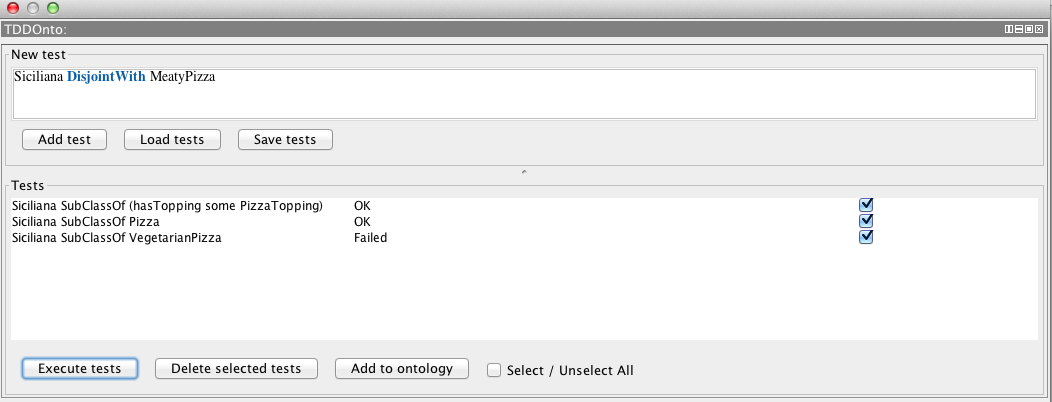
\includegraphics[width=\textwidth]{tddonto}
\end{frame}

\begin{frame}[t]{Example}
  \begin{align*}
    \oclass{Giraffe} &\osub \oclass{Herbivore} \\
    \oclass{Herbivore} &\osub \oclass{Mammal} \\
    \oclass{Mammal} &\osub \oclass{Animal}
  \end{align*}
\end{frame}

\begin{frame}[t]{Example}
  \begin{align*}
    \oclass{Giraffe} &\osub \oclass{Herbivore} \\
    \oclass{Herbivore} &\osub \oclass{Animal} \\
    \oclass{Mammal} &\osub \oclass{Animal} \\
    \\
    \oclass{Herbivore} &\onsub \oclass{Mammal}
  \end{align*}
\end{frame}
\note{
  Listing mammals misses giraffe
}

\section{New unit tests}

\begin{frame}{Available unit tests}
  \begin{itemize}
    \item TDDOnto supports few assertions
    \item Need more
  \end{itemize}
\end{frame}

\begin{frame}{New unit tests}
  \begin{itemize}
    \item Derive new tests, style of TDDOnto
    \item Prove correctness
    \item Requires formal model
  \end{itemize}
\end{frame}

\section{Benchmarking}

\begin{frame}{Benchmarking}
\end{frame}

\end{document}
